\chapter{Implementation}%Jens
Due to the agile nature of the prototype development the implementation stage begun while the design phase was still underway. This chapter describes what went into the implementation of the final prototype.

\section{Micro controllers}%Daniel
	Initially doing the implementation phase, research went into what kind of micro controller, if any, we would need to construct a working prototype. Initially we settled for an Arduino Mega 2560, but going into the production phase, we realized that an external sound source was needed. The Beaglebone Black with the Bela shield suited this purpose, and was taken in during this process.
	\subsection{Arduino}%Daniel
		The Arduino was used for handling the activation of the buttons, detecting if a mat had been pressed and activating the sounds on the Bela. 
		
	\subsection{Bela}%Jens
		Due to the sound related limitations from the Arduino Mega, we decided to add a connection to a Beaglebone with a Bela shield\footnote{Bela website: \url{https://bela.io/}}. The Bela provides a broad span of audio processing opportunities to create and manipulate audio as it is compatible with Pure Data(PD). PD is a visual programming language for multimedia that can also be used to create sounds.
		
	
\section{Code}
	\subsection{Arduino}%Daniel
		\subsubsection{Libraries}%Daniel
	\subsection{PureData}%Jens
	\begin{figure}[H]
		\centering
		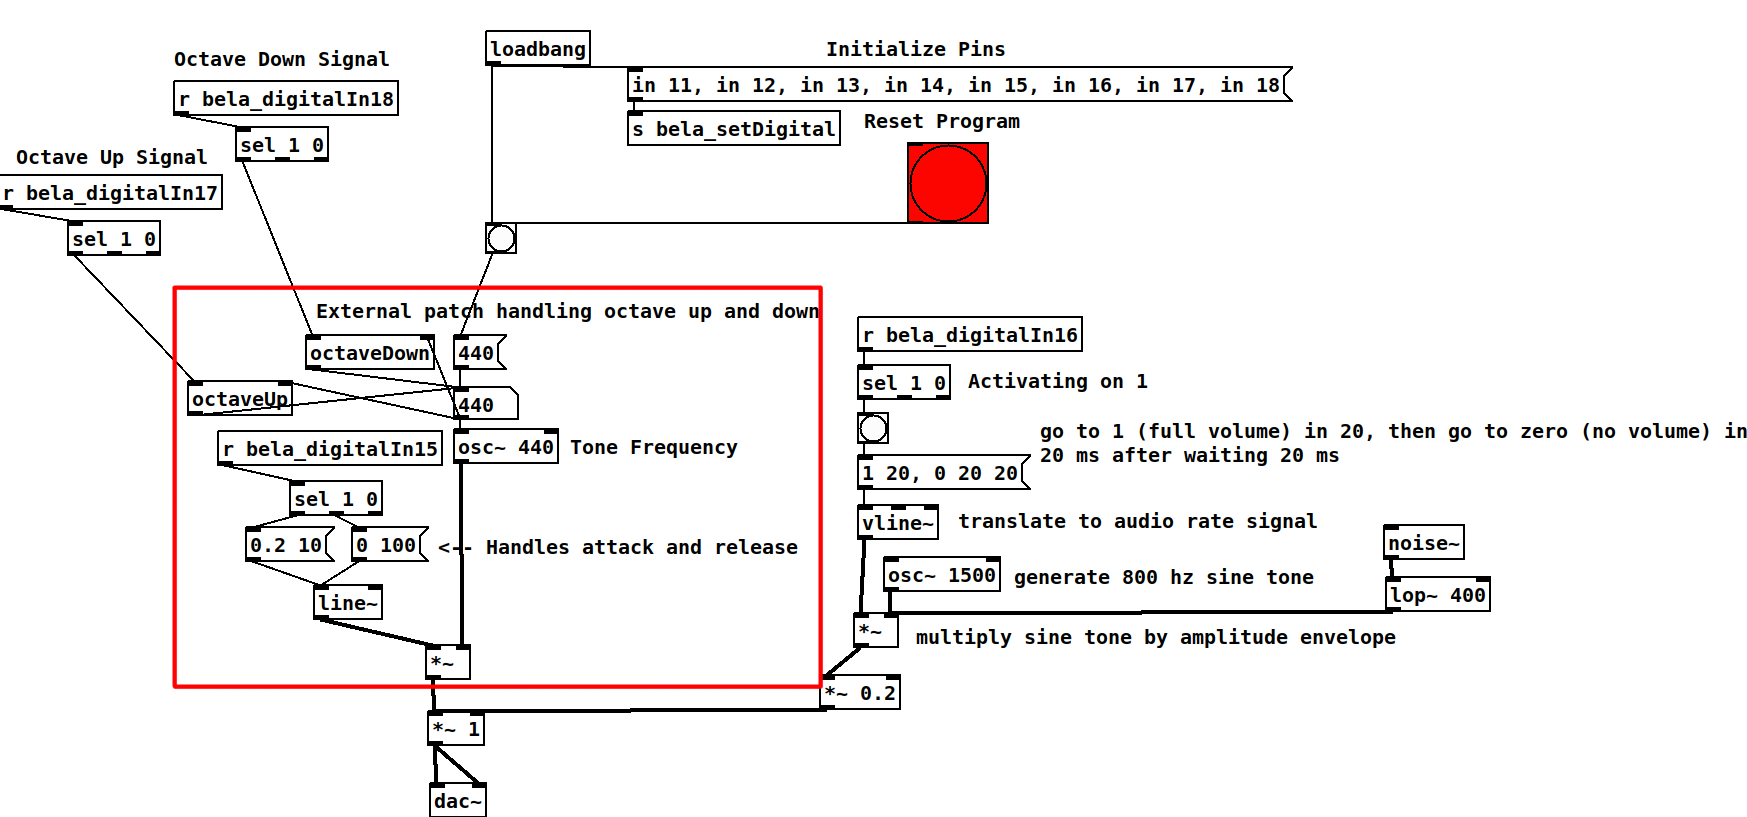
\includegraphics[width=1\linewidth]{figure/Implementation/pdPatch}
		\label{fig:pdPatch}
		\caption{Figure showing the main Pure Data patch for the prototype}
	\end{figure}	
	
\section{Circuit}


\section{The box}%Jens

	\subsection{CAD}
		
	\subsection{Assembly}

\section{The mat}%Daniel

\begin{listing}[H]
	\caption{Example 1}
	\label{listing:example1}
	\begin{minted}[frame=lines,framesep=2mm,baselinestretch=1.1,fontsize=\footnotesize,linenos]{cpp}
extern "C" __declspec( dllexport ) int init(int w, int h);
	\end{minted}
\end{listing}